\documentclass[../portafolio.tex]{subfiles}

% Solo agregue paquetes en el preámbulo de ../portafolio.tex

\begin{document}

% En esta sección, explique en detalle los siguientes aspectos:
% - Fecha de realización de la actividad
% - Título de la actividad (dentro de \section)
% - Un párrafo explicando cuál es el objetivo de la actividad
% - Nombre de personas con quien trabajó en la actividad
% - Una selección de evidencias de que usted hizo esta actividad (imágenes, códigos, respuestas a un problema teórico, etc.)
% - Una conclusión breve (qué aprendió con la actividad, qué no entendió, qué faltó trabajar, qué recomienda para futuras sesiones)

% Numero máximo de palabras en esta sección: 1000 palabras.

%%%%%%%%%%%%%%%%%%%%%%%%%%%%%%%%%%%%%%%%%%%%%%%%%%%%%%%%%%%%%%%%%%%%%%%%%%%%%%%%
\section{Ceros de una Funci\'on}   % ejemplo: Derivadas numéricas , introducción a git , 

\hfill \textbf{Fecha de la actividad:} 09 de septiembre de 2022

\medskip

%---------------------------------------------------------------------------------
% Introducción/objetivos de la actividad
En esta clase lo que hacemos el calcular los puntos en los que una funci\'on determinada se hace cero, pensando en que estamos trabajamos con funciones en $\mathbb{R}^2$ diremos que los ceros est\'an cada vez que la curva intersecta con el eje $x$. A partir de este principio, aprendimos diversos metodos para calcular dichos puntos.

%metodo de biseccion; metodo de newton; metodo de la tangente; metodo de la secante

%---------------------------------------------------------------------------------
% Con quién hizo esta actividad
Esta actividad la realic\'e de manera individual, pero recibiendo apoyo de la practicante.

%---------------------------------------------------------------------------------
% Selección de evidencias
Al trabajar los primeros incisos del laboratorio pudimos obtener la imagen \ref{img:graphceros}, donde vemos claramente el punto en el cual la funci\'on toma el valor de $x=0$, el resultado que nos entrega el codigo 

	\begin{listing}
		\begin{pythoncode}
# ~~~~~~~~~~~~~Este es el ejercicio 1.a) tomando un valor unico para betha ~~~~~~~~~~~~~~~~~~~~~~
x =np.linspace(0, np.pi/2, 100)  
b = 0.75

def u(x):
    return np.cos(x) + b*(np.sin(x))**2


def du(x, h=1e-3):
    return (u(x+h) - u(x-h))/(2*h)


plt.plot(x, du(x))
plt.hlines(0.0, 0, 1.6, colors="red")

#Este output nos entrega la funcion derivada, con la derivada en el eje "y" y los valores de x en el eje "x"


m = 0.7
n = 1.0

for i in range(10):
    c = 0.5*(m+n)
    condicion = du(m)*du(c) #Estamos buscando los ceros de la derivada, no de u(x)

    if condicion<0: 
        n = c #ya que es una de las condiciones que colocamos [a,b]---> [a,b] y el "a" lo podemos dejar solito
    else:
        m = c
		\end{pythoncode}
		\caption{Codigo utilizado para graficar la figura \ref{img:graphceros}}
		\label{code:ceros}
	\end{listing}

	\begin{figure}
		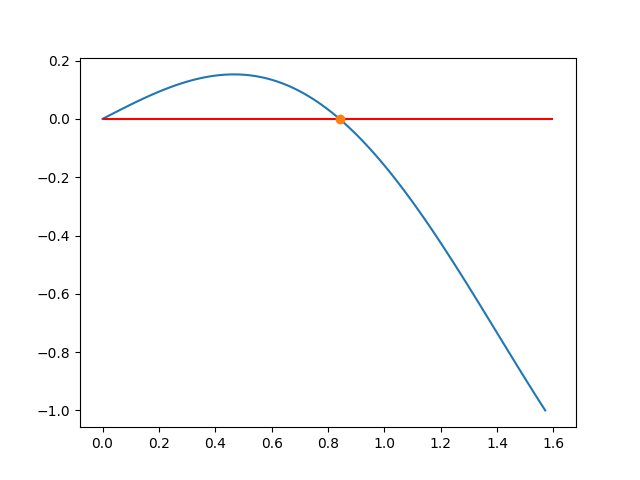
\includegraphics[scale=0.5]{graph-ceros.png}
		\caption{Gr\'afica de la primera derivada de la funci\'on $u(\theta) = \cos (\theta) + \beta \sin^2 (\theta)$}
		\label{img:graphceros}
	\end{figure}


\end{document}
